% interactapasample.tex
% v1.05 - August 2017
%This template is for authors who are preparing a manuscript for a Taylor \& Francis journal using the \LaTeX\ document preparation system and the \texttt{interact} class file, which is available via selected journals' home pages on the Taylor \& Francis website.
%The \textsf{Interact} layout style allows for five levels of section heading, all of which are provided in the \texttt{interact} class file using the standard \LaTeX\ commands \verb"\section", \verb"\subsection", \verb"\subsubsection", \verb"\paragraph" and \verb"\subparagraph". Numbering will be automatically generated for all these headings by default.
%August 2021 - This interactsample.tex template has been edited to meet the Data Science Journal guidelines for Research Papers. -- WDS-ITO ito-ra1@oceannetworks.ca
%%%%%%%%%%%%%%%%%%%%%%%%%%%%%%%%%%%%%%%%%%%%%%%%%%%%%%%%%%%%%%%%%%%%%%%%%%%%%%
\documentclass{interact}
\usepackage[utf8]{inputenc}
\usepackage[T1]{fontenc}
\usepackage{graphicx}
\usepackage{rotating}
\usepackage{pgfplots}
\pgfplotsset{width=12cm,height=20cm,compat=1.18}
\usepackage[caption=false]{subfig}% Support for small, `sub' figures and tables
%\usepackage[nolists,tablesfirst]{endfloat}% To `separate' figures and tables from text if required
%\usepackage[doublespacing]{setspace}% To produce a `double spaced' document if required
%\setlength\parindent{24pt}% To increase paragraph indentation when line spacing is doubled
\usepackage{array}% http://ctan.org/pkg/array
\usepackage[style=authoryear-ibid,backend=bibtex,bibencoding=utf8,dashed=false]{biblatex}% Manages references that are imported via \addbibresource. Notes format was also altered. backend=biber,
\addbibresource{references.bib}
\renewcommand*{\postnotedelim}{\addcolon\space}
\DeclareFieldFormat{postnote}{#1}
\DeclareFieldFormat{multipostnote}{#1}
\usepackage{subfiles}% Manages the appendix (a separate .tex file)
\graphicspath{{images/}}
\usepackage{enotez}% Renders footnotes as endnotes to meet DSJ's guidelines
\usepackage{hyperref}
\hypersetup{
 colorlinks=true,
 linkcolor=blue,
 filecolor=blue,  
 urlcolor=blue,
 citecolor=blue
 }
\begin{document}
\articletype{Research Article}% Specify the article type or omit as appropriate
\title{\huge Harvestable Metadata Services Development\\\large Analysis of Use Cases from the World Data System}
\author{\name{Alicia Urquidi D\'iaz,\textsuperscript{a}\textsuperscript{b}\thanks{Corresponding author: Alicia Urquidi D\'iaz, alicia.urquidi@utoronto.ca. For inquiries about WDS-ITO or the HMetS-WG, please contact Karen Payne, ito-director@oceannetworks.ca.}
Robert R. Downs,\textsuperscript{c}
Qi Xu,\textsuperscript{d}\textsuperscript{e}
Juanle Wang,\textsuperscript{f}\textsuperscript{g}
Aude Chambodut,\textsuperscript{h}\textsuperscript{i}
Liu Chuang,\textsuperscript{j}
Sarah Reay,\textsuperscript{k}\textsuperscript{l}
Karen Payne.\textsuperscript{a}}
\affil{\textsuperscript{a}World Data System - International Technology Office, Canada;
\textsuperscript{b}Scholars Portal, Canada; 
\textsuperscript{c}NASA Socioeconomic Data and Applications Center, United States; 
\textsuperscript{d}National Space Science Data Center, China;
\textsuperscript{e}National Space Science Center, Chinese Academy of Sciences;
\textsuperscript{f}WDC-Renewable Resources and Environment, China;
\textsuperscript{g}Institute of Geographic Sciences and Natural Resources Research, Chinese Academy of Sciences;
\textsuperscript{h}International Service of Geomagnetic Indices;
\textsuperscript{i}Centre de Donn\'ees astronomiques de Strasbourg, France;
\textsuperscript{j}Global Change Data Publishing and Repository, China;
\textsuperscript{k}WDC-Geomagnetism (Edinburgh), UK;
\textsuperscript{l}INTERMAGNET.}}
\maketitle
%The "\thanks" command may be used to create additional footnotes to the title or authors' names if required. 

\begin{abstract}
Minimally, a research data repository exists to make a collection of data assets available to potential users. If a dataset cannot be discovered and found, it cannot be reused \parencite{garnett_open_2017}. Harvestable metadata catalogues are a key strategy for achieving greater global findability of data assets, as they create a surveyable access point to discover data products within large data collections. Such catalogues can be especially effective if they are tailored for interoperability with feature-rich infrastructures (e.g. meta-catalogues, see \cite{elman_making_2020, crfcb_metacatalogue_2014}) that are highly visible and widely used, and also themselves integrated within the larger ecosystem of research infrastructures.

This study offers insight into a set of World Data System (WDS) research data repositories’ ongoing and successful implementations of harvestable metadata services, which apply established and emerging research data standards and practices to fit global, local and domain-specific interoperability contexts. Establishing a harvestable metadata service involves making choices in a space where standards and technologies are continuously evolving. The repositories in this study leverage the resources they have, within the policy and funding constraints of their institution, to serve the changing needs of heterogeneous user groups.
This document encapsulates and completes the work that was carried out by the WDS International Technology Office (ITO) Harvestable Metadata Services Working Group (HMetS-WG). \end{abstract}

\begin{keywords}
Metadata harvesting, metadata for discovery, World Data System, metadata catalogue, dataset findability
\end{keywords}

\section{Introduction}\label{intro}
Harvestable metadata services are an effective, established and widely-used approach to promoting data discovery and sharing across broad communities of potential data users, across multiple disciplines \parencite{lokers_analysis_2016, valentine_earthcube_2020}. For the purpose of this study, we understand harvestable metadata as \emph{a set of metadata records in a standardized format and schema that is shared with aggregation services by means of specific protocols for metadata transfer, which are also standardized}. In this paper, we describe examples of ongoing and successful implementations of harvestable metadata services, which apply emerging and established standards and community practices to fit local and domain-specific research data management contexts. These use cases originated from the Harvestable Metadata Services Working Group (HMetS-WG)\endnote{The group was led by the International Technology Office\endnote{WDS-ITO, \href{https://wds-ito.org}{https://wds-ito.org}.} of the International Science Council's (ISC) World Data System (WDS).}, which met in a series of working sessions over 6 months during 2020. The study aims to give an overview of the infrastructures, standards and communities of the members of the WG, as well as engaging in a wider-ranging discussion of challenges that repository managers may face in developing data services such as harvestable metadata.

Designed as a qualitative study, this paper explores the issues surrounding the implementation of harvestable metadata services. We start with a description of use cases, with a focus on each repository's technical features, along with the challenges encountered in pursuit of self-defined and community-oriented service development goals. Repositories are also characterized by the subject and disciplinary areas covered, targeted user groups, and services offered. The full-length profiles for each platform are available as a separate publication \parencite{urquidi_diaz_harvestable_2022}. After examining the use cases within the context of the current literature on best practices for metadata syndication and pathways toward interoperability, we present a set of lessons learned from the experiences reported by the repositories in this study. These experiences involved making decisions about which technologies to develop for an often heterogeneous dynamic user base, within an evolving technological landscape, in order to implement data and metadata services that fit within the resource and policy constraints of the repository.

\subsection*{Metadata harvesting, standards and protocols}\label{subintro}
In a typical metadata sharing process, a research data repository will share a catalogue of assets: a collection metadata records that describe each dataset, typically via a search interface on the repository's portal. The repository may also share a set of standardized metadata records via additional access points (or harvestable metadata services), using a metadata transfer protocol through which aggregation services, such as harvesters, obtain the metadata (see Fig. \ref{image-harvesting}). Permanent links to data landing pages at the host repository are typically contained in those records. An aggregator may then convert (re-format or cross-walk) the acquired records into a unified display standard, to be disseminated by means of a federated metadata catalogue or a federated search engine. Examples of metadata harvesters that target research data include the Canadian Federated Research Data Repository (FRDR),\endnote{Federated Research Data Repository (FRDR), \href{https://www.frdr-dfdr.ca/repo/.}{https://www.frdr-dfdr.ca/repo/}.} and B2FIND (Europe).\endnote{EUDAT Collaborative Data Infrastructure - B2FIND, \href{https://eudat.eu/services/b2find}{https://eudat.eu/services/b2find}.}

The adherence to shared standards and community practices is a key tenet for successful digital research infrastructure (DRI) integration and interoperability \parencite{dietze_iterative_2018, yu_coevolution_2021, waide_demystifying_2017}. Common standards for harvestable metadata include the Dublin Core \parencite{dcmi_dublin_2020}, DataCite \parencite{datacite_metadata_working_group_datacite_2019} and ISO 19115 \parencite{iso_iso_2019} metadata schemas, as well as transfer protocols such as OAI-PMH \parencite{lagoze_open_2015} and OGC-CSW \parencite{nebert_ogc_2016}. Metadata records are usually transferred as eXtensible Markup Language (XML) or JavaScript Object Notation (JSON, and JSON-LD, for linking data within semantic metadata) files.  Another approach to syndicating metadata uses semantic metadata tags, such as Schema.org,\endnote{Schema.org, \href{https://schema.org/}{https://schema.org/}.} that are placed in the HTML of dataset landing pages on a repository's web portal, or in separate metadata files. This strategy relies on web crawlers (such as Google) parsing the semantic metadata to aggregate and index the landing pages for search engine retrieval. Even though this approach to metadata sharing can complement harvestable metadata services, the semantic strategy was not tackled by the HMetS-WG. Instead, WDS-ITO engaged members of various communities in a separate initiative to develop semantic metadata using Schema.org \parencite{payne_how_2022}.

As the importance of reusing data is increasingly recognized across disciplines, data repositories have proliferated to meet this demand, with the number of data repositories listed in registries such as re3data\endnote{The Registry of Reserarch Data Repositories, \href{https://www.re3data.org/}{https://www.re3data.org/}, is a global registry of of research data repositories.} growing rapidly \parencite{culina_navigating_2018}. As each data repository offers additional open data products, finding a particular dataset of interest becomes challenging for potential data users \parencite{kramer_data_2018, plante_implementing_2021}. A recognized approach to address this challenge is for repositories to establish capabilities for harvesting metadata to facilitate searchability and global discoverability \parencite{culina_navigating_2018, plante_implementing_2021, wu_data_2019}. Furthermore, the availability of harvestable metadata is an indicator of dataset findability \parencite{coretrustseal_coretrustseal_2019, fair_data_maturity_model_wg_fair_2020} and a measure of repository TRUST-worthiness because it entails better integration with the wider data management community \parencite[3]{lin_trust_2020}.

\begin{figure}
\centering
\includegraphics[width=1\columnwidth]{BeingFound_Repository.png}
\caption{The metadata harvesting process. Standardized metadata is harvested from repository catalogues, then processed, by an aggregation service. The service disseminates the metadata records through a search and discovery portal, and/or by serving it to further aggregation services for distribution.} \label{image-harvesting}
\end{figure}

\section{Research Methodology}\label{method}
The study's methodology included both top-down and bottom-up approaches to data collection and analysis. The focus of the Harvestable Metadata Services Working Group was on exposing the metadata assets of the WDS community, and its main goals were to facilitate WDS repository maturation through support for harvestable metadata services development, and an increase in findable and accessible data from WDS members. The Working Group was conceived as "a community-driven, multidisciplinary platform where WDS Members can interact, collaborate, and share their good practices, approaches, and pain-points associated with creating harvestable metadata services. The intent is to first identify the issues that are preventing WDS Members from exposing their metadata assets, create a scope of work detailing the issues identified, then create and follow through with an implementation plan to create publically harvestable metadata services using common and well established protocols." \parencite{}


Deliverables and Milestones

The Harvestable Metadata Services WG aims to help participants to:

    Determine if they want to create an implementation plan to create a harvestable metadata service, and if so
    Examine the current state of their metadata and metadata delivery options.
    Work with colleagues to write a scope of work that will enable them to create a harvestable metadata service.
    Include some sort of consumption benchmark in the plans, a metric of how much metadata and data they are currently serving—the 'hits' their data is getting—and a method to compare this number against the amount of metadata and data they are serving, or the clients they are reaching after implementing a harvestable metadata service.
    Include consumption options in the plans—a list of which harvesters they can support.
    Collectively gather all of the use cases, identify common pain-points and lessons learned, and publish as guidance for the wider Research Data Management community who are facing the same challenges.
    Support participants in their implementation and where necessary, seek additional expertise and resources to support WG member implementation.



By the end of this 24-month WG period, there will be:

    An acceleration in the maturation of less advanced WDS communities, and the emergence of a global community supporting scientific data services.
    An explicit understanding of the barriers to metadata service deployment in a variety of contexts and settings.
    An increase in WDS Members with harvestable metadata services, and by extension, more findable and accessible data. This will increase the global standing of WDS as an integral part of international collaborative scientific research.
    Users and consumers of these services accessing data that was previously unavailable.



In September 2019, the WDS-ITO invited WDS members to participate in the HMetS-WG and to (optionally) serve as use cases for the study. The invitation was sent to 35 unique WDS member organizations that had previously expressed interest in being informed about new WDS initiatives. Nine repositories participated in the group, and seven (Table \ref{table-subjects}) were adopted as use cases. 

The group's work agenda was initially guided by a workflow structure proposed by WDS-ITO (Fig. \ref{flowchart}), which represents harvestable metadata services development as a set of discrete, successive steps. As the group progressed, WDS-ITO provided members with an enhanced package of resources, which included a Harvestable Metadata Services Implementation Plan template \parencite{urquidi_diaz_template_2021}. This resource borrowed heavily from the CESSDA-Saw guidance package \parencite{bornatici_cessda_2017} and JISC project plan templates \parencite{jisc_jisc_2011} for data service planningm, which were designed to be adapted to specific use cases—to a single service or subset of services (such as harvestable metadata services)—and include guidance on drafting implementation plans for these services. Supporting information resources in this package also included a Twine interactive narrative/storyfied walk-through of the implementation plan flow-chart \parencite{li_interactive_2021}, and a Zotero library with references to other digital resources related to harvestable metadata services \parencite{urquidi_diaz_zotero1_2021, urquidi_diaz_zotero2_2021}. 

\subsection*{Data Collection}\label{data_collection}
In the first few sessions, repositories were asked to present an overview of their infrastructure, data holdings, and services. All participating repositories provided the group with a schematic overview of their features and three repositories (NSSDC, INTERMAGNET and SEDAC) completed the implementation plan template and shared ith with WDS-ITO. 





\subsection*{Data Processing and Analysis}\label{data_processing}


We used the sources of information mentioned above in section \ref{data_collection} to complile detailed repository profiles that were published separately on Zenodo as supplementary materials \parencite{urquidi_diaz_harvestable_2022}. Wherever available, the summary profiles reference repositories' technical documentation and other relevant publications. 

The following sections were covered:

\begin{enumerate}
\item Institutional overview: Brief description of the repository's institutional context: Its governance, history, mandate, mission, memberships, and other organizational features.
\item User community: Target communities for repository services.
\item Infrastructure overview: Description of repository's data holdings and technical infrastructure for service provision.
\item Current state of metadata: Metadata formats, standards used, and metadata services (if any).
\item Planned development: Plans for future development.
\item Resources: Description of repositories' sources of support and financing.
\item Challenges: Initially, each repository described the challenges they have faced in developing harvestable metadata and other data services on their platforms.
\end{enumerate}

Table \ref{summary} presents some basic facts about each repository, and Table \ref{table-subjects} describes the subject areas covered by the data collections and the target user groups for each repository.

\begin{figure}
\centering
\includegraphics[width=1\columnwidth]{flowchart.jpg}
\caption{Flow-chart diagram of a typical harvestable metadata services implementation \parencite{payne_2021}. This diagram gives a schematic representation of the steps involved in creating a harvestable metadata service. The HMetS-WG used these steps to scaffold the group's initial work.} \label{flowchart}
\end{figure}

In section \ref{data_processing} we described the process through which the individual repository profiles were put together from varied sources of information, including WG members' own extensive contributions. After those profiles had been completed, the group gathered to identify the common threads and challenges reported in the uses cases, and possible approaches to tackling those challenges were explored. These discussions took place during synchronous Zoom meetings that were facilitated by WDS-ITO.

In one session, the group analyzed the challenge statements that were reported in each of the individual use cases. In a first step, the group used colours to propose categories into which the original statements could be synthesized (see Figure \ref{challenges-sorting} for an illustration of this coding exercise). Through further analysis and discussion the group identified three major overarching themes, or common sources, for the challenges reported: changing user needs, sustainability, and evolving technologies. 


\section{The HMetS-WG Set of Use Cases}\label{use-cases}
\subsection{Repositories participating in the working group}\label{participants}
The participating institutions (see Table \ref{table-institutions}) were based in China, the UK, the US, and France. Seven repositories were Regular\endnote{``[O]rganizations that are data stewards and/or data analysis services (e.g., data centres and services that support scientific research by holding and providing data or data products).'' \parencite{wds_scientific_committee_icsu-wds_2016}.} Members of WDS and two were Network\endnote{``[U]mbrella bodies representing groups of data stewardship organizations and/or data analysis services, some of which may or may not be WDS Regular Members” who “usually serve as coordinating agents for nodes that have common characteristics and mostly common disciplines.'' \parencite{wds_scientific_committee_icsu-wds_2016}.} Members. 

\begin{table}
\tbl{HMetS-WG attendees, with WDS membership type and host institutions.}
{\renewcommand{\arraystretch}{1.5}{\begin{tabular}{p{0.35\linewidth} p{0.1\linewidth} p{0.55\linewidth}}\\\hline
WDS Member & Type & Host institution(s)\\
\hline
Centre de Donn\'ees Astronomiques de Strasbourg (CDS) & Regular & Strasbourg Astronomical Observatory (ObAS); University of Strasbourg; French National Centre for Scientific Research (CNRS)\\
Global Change Research Data Publishing and Repository (GCdataPR) & Regular &Institute of Geographical Sciences and Natural Resources Research (IGSNRR), Chinese Academy of Sciences (CAS); Geographical Society of China\\
International Real-time Magnetic Observatory Network (INTERMAGNET) & Network & Multiple institutions (worldwide)\\
International Service of Geomagnetic Indices (ISGI) & Regular & School and Observatory of Earth Sciences (EOST); University of Strasbourg; French National Centre for Scientific Research (CNRS)\\
International GNSS Service (IGS) & Network & Multiple institutions\\
National Space Science Data Center (NSSDC) & Regular & National Space Science Center (NSSC), Chinese Academy of Sciences (CAS)\\
Socioeconomic Data and Applications Center (SEDAC) & Regular & Center for International Earth Science Information Network (CIESIN), Columbia University; Earth Observing System Data and Information System (EOSDIS), National Aeronautics and Space Administration (NASA).\\
World Data Center for Geomagnetism (Edinburgh) & Regular & British Geological Survey (BGS)\\
World Data Centre for Renewable Resources and Environment (WDC-RRE) & Regular & IGSNRR; CAS\\ \bottomrule
\end{tabular}}}
%\tabnote{\textsuperscript{a}This footnote shows how to include footnotes to a table if required.}
\label{table-institutions}
\end{table}

\subsection{Subject areas and target user communities}\label{subjects}
The research areas served represent a predominant earth- and planetary sciences orientation. Social sciences, including environmental and economic sciences, were also strongly represented. Three uses cases can be classified broadly as social and environmental science research centers that focus on spatial data: The World Data Centre for Renewable Resources and the Environment (WDC-RRE),\endnote{World Data Centre for Renewable Resources and Environment, \href{http://wdcrre.data.ac.cn/}{http://wdcrre.data.ac.cn/}.} Global Change Data Publishing \& Repository (GCdataPR)\endnote{Global Change Research Data Publishing and Repository, \href{http://www.geodoi.ac.cn/weben/}{http://www.geodoi.ac.cn/weben/}.} and the Socioeconomic Data and Applications Center (SEDAC).\endnote{Socioeconomic Data and Applications Center, \href{https://sedac.ciesin.columbia.edu/}{https://sedac.ciesin.columbia.edu/}.} Two repositories, the Chinese National Space Science Data Centre (NSSDC)\endnote{National Space Science Data Center of China, \href{https://www.nssdc.ac.cn/eng/}{https://www.nssdc.ac.cn/eng/}.} and the International GNSS Service (IGS)\endnote{International GNSS Service, \href{https://igs.org/}{https://igs.org/}.} provided uses cases for astronomy and geodesy. Lastly, the International Real-time Magnetic Observatory Network (INTERMAGNET)\endnote{International Real-time Magnetic Observatory Network, \href{https://intermagnet.github.io/}{https://intermagnet.github.io/}.} and the International Service of Geomagnetic Indices (ISGI)\endnote{International Service of Geomagnetic Indices, \href{http://isgi.unistra.fr/}{http://isgi.unistra.fr/}.} are dedicated to the management and sharing of geomagnetic research data and data products.

\begingroup
\setlength{\tabcolsep}{6pt} % Default value: 6pt
\renewcommand{\arraystretch}{1.5} % Default value: 1
\begin{table}
\tbl{Subject areas represented by repositories in the use cases and target users groups for each repository. Subject tags were provided to WDS-ITO by the repositories themselves.}
{\renewcommand{\arraystretch}{1.5}{\begin{tabular}{p{0.17\linewidth} p{0.42\linewidth}p{0.41\linewidth}}\\\hline
Repository & Subject tags & User groups\\
\hline
GCdataPR & Earth sciences, Economics, Geography, Agriculture, Environmental studies and forestry, History, Area studies, Geo-ecosystems & Global change researchers in China and worldwide \\
IGS & Space sciences, Earth sciences, Geodesy, GPS, GNSS, Precise positioning, navigation, and timing & Mainly IGS staff, project and working group participants. More broadly: worldwide users of modern mapping, orientation and navigation systems, enterprises, non-profits, institutions and government actors\\
INTERMAGNET & Earth sciences, Geomagnetism, Space sciences & Scientific community, geomagnetism community, members of IAGA,\endnote{International Association of Geomagnetism and Aeronomy, \href{http://www.iaga-aiga.org/}{http://www.iaga-aiga.org/}.} commercial users.\\
ISGI & Solar-Terrestrial physics, Space weather-Space Climate, Space sciences, Earth sciences, Geomagnetism & Academia (including behavioural biology), members of IAGA communities, private and public sectors (military, telecommunications, satellite operators)\\
NSSDC & Astronomy, Space sciences, Computer sciences, Space physics, Space weather, Planetary science & Typical users are Chinese and international researchers in subject areas\\
SEDAC & Earth sciences, Chemistry, Cultural and ethnic studies, Economics, Geography, Political science, Sociology, Computer sciences, Statistics, Systems science, Agriculture, Architecture and design, Business, Engineering, Environmental studies and forestry, Health sciences, Transportation, Anthropology, Area studies, Environmental science, Sustainability science, Climate science, Information system science & User community is interested in studying human interactions in the environment\\
WDC-RRE & Earth sciences, Geography, Environmental studies and forestry, Natural resources, Ecology, Geoinformatics & Mainly academic researchers and students, also scientific staff and technicians, general public, government agencies, policy makers, international organizations \\ \bottomrule
\end{tabular}}}
\label{table-subjects}
\end{table}
\endgroup

\subsection{Repository features}\label{features}
Table \ref{summary} gives an overview of each repository's technical features: the type of repository platform and catalogue service used, metadata standards and protocols, any added services, and a list of any current, known aggregators of their metadata assets. Figure \ref{wds-survey} presents the metadata exchange protocols utilized by the repositories studied, in the context of those of the larger WDS membership (as surveyed in 2019 by WDS-ITO \parencite{payne_world_2020}). Relative to WDS members previously surveyed, our use cases have (or plan to develop) more OGC-CSW and Opensearch, and fewer OAI-PMH services. It also must be noted that the earlier WDS member survey data does not distinguish between protocols residing within repositories and those that are provided by aggregators who disseminate metadata on behalf of repositories (e.g. EOSDIS or GEOSS).

\subsubsection{Participation in research data networks}
As we shall see below, it appears that participation in national, regional, as well as subject-specific networks has generally shaped repositories' infrastructure, particularly the ways in which their adoption of harvestable metadata services has developed or will be developed in the near future.

All studied repositories have been guided or supported by a larger entity while developing harvestable metadata services: INTERMAGNET and ISGI have participated in the European Open Science Cloud's (EOSC) EPOS ERIC project, while WDC-RRE, NSSDC and GCdataPR have developed with support from Chinese research data institutions. Finally, both SEDAC's and IGS's infrastructures have been supported by the National Aeronautics and Space Administration’s (NASA) Earth Observing System Data and Information System's (EOSDIS) community, and their extensive collections of knowledge and technical resources.

\begingroup
\setlength{\tabcolsep}{6pt} % Default value: 6pt
\renewcommand{\arraystretch}{1.5} % Default value: 1
\begin{sidewaystable}
\tbl{Use Case Infrastructures: Summary of Features}
{\begin{tabular}{p{0.105\linewidth} p{0.15\linewidth} p{0.165\linewidth} p{0.16\linewidth} p{0.10\linewidth} p{0.16\linewidth} }\\\hline
& Repository platform\newline \& catalogue & Metadata standards & Metadata service protocols & Added services & Known aggregators\\\hline
GCdataPR & Custom & DCI\endnote{Data Citation Index, \href{https://clarivate.com/webofsciencegroup/solutions/webofscience-data-citation-index/}{https://clarivate.com/webofsciencegroup/solutions/webofscience-data-citation-index/}.}, DataCite & OpenSearch & Real-time usage statistics & CrossRef, China-GEOSS, China National Knowledge Infrastructure (CNKI), DCI (metadata shared via email)\\
IGS & Catalogue via NASA CMR \newline \emph{- State-of-the-art IGS data discovery platform in development} & DIF 10, ECHO 10, ISO 19115-2:2009 (MENDS and SMAP dialects), UMM-C & CMR CSW, CMR public APIs, OpenSearch & \emph{- In development} & via NASA's CMR\\
INTERMAGNET & Custom repository with some datasets on GFZ Potsdam's data repository & Via INTERMAGNET: IAGA2002, CDF; Via GFZ: GeoJSON, DataCite, ISO 19115 & Via homepage: HTTP, FTP; Via GFZ: request to DataCite's API & none reported & DataCite, FIDGEO\endnote{Specialized Information Service for Geosciences, \href{https://www.fidgeo.de/en/fid-geo-en/}{https://www.fidgeo.de/en/fid-geo-en/}.}\\
ISGI & Custom \newline \emph{- Public access metadata service} & IAGA2002 \newline \emph{- CERIF, DataCite and/or DCAT based profiles and/or crosswalks} & Via homepage: HTTP; request to DataCite’s API & none reported\\
NSSDC & Custom & NSSDC Core Metadata Specification, SPASE \newline \emph{- DataCite, VO Data model} \newline \emph{- DataCite-NSSDC schema compatibility} & OpenSearch, OGC-CSW (via WDS China), Data search platform, \newline \emph{- OAI-PMH} & DOI, Handle, CSTR IDs \newline \emph{- Metadata registration service} & National Science and Technology Data Sharing Network of China, Scientific Data Center of Chinese Academic of Sciences\\
SEDAC & Vital Digital Asset Management System (Fedora) \newline \emph{- Migration to Drupal 8 underway} & FGDC CSDGM, ISO19115, DataCite & International Data Network's OGC CSW, NASA's CMR CSW, CMR public APIs, OpenSearch & none reported & DataCite, GEOSS (via EOSDIS/CMR)\\
WDC-RRE & Custom: Debian OS, OSS NGNIX, PostgreSQL, TorCMS & Dublin Core, ISO 19115, WDC-RRE’s Data Identification and Metadata standards \newline \emph{- New metadata specification planned} & OpenSearch, OGC-CSW 3.0.0, OAI-PMH 2.0, SRU 1.1., \newline \emph{- Geonetwork} & PID versioning for dynamic datasets & WDS-China, CNKI\\
\bottomrule
\end{tabular}}
\tabnote{\textsuperscript{i}Features given in \emph{italics} are planned or currently in development.;\newline \textsuperscript{ii}This use case includes both INTERMAGNET and its host organization, WDC-Geomagnetism (Edinburgh)} 
\label{summary}
\end{sidewaystable}
\endgroup

\begin{figure}
\centering
\textbf{Metadata aggregation and syndication mechanisms\\ reported by WDS and HMetS-WG members}\par\medskip
% Bar charts - uses package pgfplots
% Author: Stefan Kottwitz
% https://www.packtpub.com/hardware-and-creative/latex-cookbook
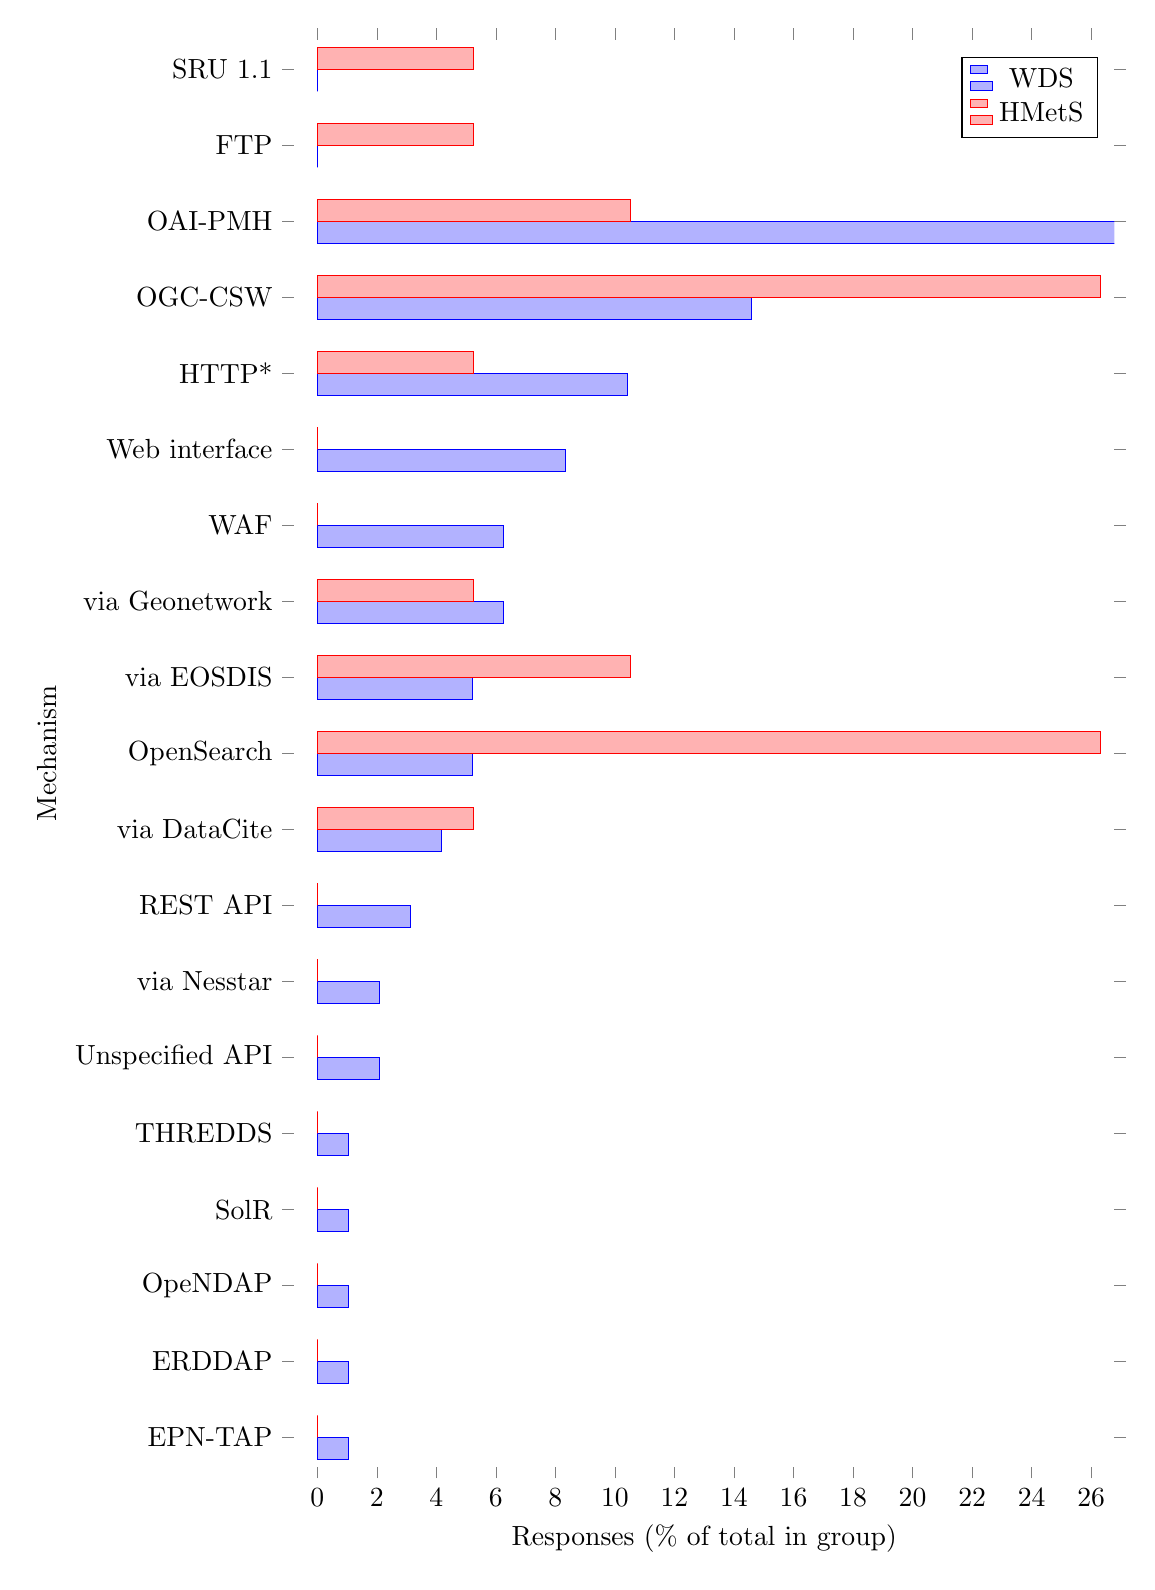
\begin{tikzpicture}
\pgfplotbarshift
  \begin{axis}[
   xbar = 0pt,
   ylabel = Mechanism,
   xlabel = Responses (\% of total in group), 
xmin=0,xmax=26,
symbolic y coords = {EPN-TAP,ERDDAP,OpeNDAP,SolR,THREDDS,Unspecified API,via Nesstar,REST API,via DataCite,OpenSearch,via EOSDIS,via Geonetwork,WAF,Web interface,HTTP*,OGC-CSW,OAI-PMH,FTP,SRU 1.1},
bar width=8pt,
ymin = {[normalized]0}, ymax = {[normalized]18},
enlargelimits = 0.03,
y axis line style = { opacity = 0 },
x axis line style = { opacity = 0 }
]
\addplot coordinates {(1.041666667,EPN-TAP)
(1.041666667,ERDDAP)
(1.041666667,OpeNDAP)
(1.041666667,SolR)
(1.041666667,THREDDS)
(2.083333333,Unspecified API)
(2.083333333,via Nesstar)
(3.125,REST API)
(4.166666667,via DataCite)
(5.208333333,OpenSearch)
(5.208333333,via EOSDIS)
(6.25,via Geonetwork)
(6.25,WAF)
(8.333333333,Web interface)
(10.41666667,HTTP*)
(14.58333333,OGC-CSW)
(27.08333333,OAI-PMH)
(0,FTP)
(0,SRU 1.1)};
\addplot coordinates {(0,EPN-TAP)
(0,ERDDAP)
(0,OpeNDAP)
(0,SolR)
(0,THREDDS)
(0,Unspecified API)
(0,via Nesstar)
(0,REST API)
(5.263157895,via DataCite)
(26.31578947,OpenSearch)
(10.52631579,via EOSDIS)
(5.263157895,via Geonetwork)
(0,WAF)
(0,Web interface)
(5.263157895,HTTP*)
(26.31578947,OGC-CSW)
(10.52631579,OAI-PMH)
(5.263157895,FTP)
(5.263157895,SRU 1.1)};
  \legend{WDS,HMetS}
  \end{axis}
\end{tikzpicture}
\caption{This bar chart compares the mechanisms for metadata exposure (aggregation, discovery, etc.) that were reported by the HMetS-WG repositories with those reported by WDS repositories in a 2019 member survey \parencite[11, 15]{payne_world_2020}. Because some repositories reported serving their metadata \emph{via} third-party services, we have included those services as well (e.g. DataCite, EOSDIS, etc.). \textsuperscript{*}Includes schema.org.}\label{wds-survey}
\end{figure}

\medskip
\noindent \textbf{Geomagnetism data in Europe: the EPOS ERIC.}
Within the European geomagnetism community, the European Plate Observing System European Research Infrastructure Consortium (EPOS ERIC) has played an important role promoting the uptake of 21st century technologies and standards to create more granular and robust metadata and dataset documentation \parencite{chambodut_geomagnetic_2018, flower_epos_2019}. Following EPOS ERIC's leadership, ISGI plans to migrate the repository's metadata records into an interoperable schema that will allow repositories to serve metadata to European aggregators like OpenAIRE. Currently, ISGI is considering implementing CERIF, DataCite, and/or DCAT compliant metadata. Since 2013, INTERMAGNET has been publishing yearly definitive data through the GEZ (GeoForschungsZentrum) Data Service, which serves dataset metadata to aggregators using various metadata standards and sharing protocols.

\medskip
\noindent \textbf{The Chinese research data infrastructure.}
GCdataPR, NSSDC and WDC-RRE belong to the original Chinese data repositories that joined the ICSU system of World Data Centers in 1988. In 2008, to promote collaboration between the eight Chinese repositories at WDS, the WDS China Common Clearinghouse\parencite{wds-china_introduction_2017} was created. The prototype for WDS China's unified metadata search portal was built using Pycsw, a Python implementation of the OGC's Catalogue Services for the Web (CSW) standard \parencite{wang_progress_2020}. This initiative, which was led by WDC-RRE, encouraged and supported WDS members to develop harvestable metadata services based on similar spatial data interoperability standards, notably ISO 19115/19139/19119 metadata and the OGC CSW protocol.
Outside of WDS, the Chinese repositories form part of the larger Chinese digital research infrastructure as part of 20 Chinese Data Centers organized under the National Science and Technology Infrastructure Center of China.\endnote{Many of which also maintain a close collaboration with WDS as non-members.} The 20 data centers provide their metadata collections on a regular basis to a unified metadata search portal operated by the National Science and Technology Data Sharing Network of China \parencite{nsti_china_2021}. These records must comply with the Chinese Science and Technology Infrastructure – Resource Core Metadata standard(GB/T 30523-2014, \cite{china_national_institute_of_standardization_gbt_2014}). Both, WDC-RRE and NSSDC maintain custom metadata profiles that integrate local and international interoperability features.

\medskip
\noindent \textbf{EOSDIS at NASA.}
Two of the repositories, SEDAC and IGS, are (at least partially) based in the United States, and they enjoy support from the National Aeronautics and Space Administration's (NASA) infrastructure. 
As one of NASA’s Distributed Active Archive Centers (DAACs), SEDAC participates actively in initiatives stewarded by the Earth Science Data and Information System (ESDIS) project and SEDAC metadata is provided to NASA’s Earth Observing System (EOS) Common Metadata Repository (CMR). The CMR is the back-end of Earthdata Search, the Global Change Master Directory (GCMD) and the International Data Network (IDN), the latter of which transfers SEDAC metadata into GEOSS. 
The complete collection of IGS data, which is distributed across data centres, has one of two complete mirrors hosted by a NASA EOSDIS data center, the Crustal Dynamics Data Information System (CDDIS) (the second mirror is hosted by the European Space Agency).\endnote{Since 2018, the European Space Agency (ESA) GNSS Science Support Centre (GSSC), located in Madrid started an initiative to create additional mirrors, in a project that also contemplates a new service platform: the IGS Global Data Centre \parencite{gssc_igs_2021}.} Thus, at present, metadata records for SEDAC datasets and for IGS collections are served in metadata search/retrieval endpoints at the CMR \parencite{noll_cddis_2019}, and they are available in multiple established metadata formats, specifically: DIF 10, ECHO 10, ISO 19115-2:2009 (MENDS and SMAP dialects), and UMM-C \parencite{reiter_cmr_2019}.

\section{Challenges}\label{discussion}
The first major theme reflects repositories' efforts to track and meet the changing needs of the user community, adopting standards that maximize metadata interoperability, with metadata schemas that are widely used, but also versatile and extensible. Serving the needs of data users is one of the main missions of research data repositories, and it is a key indicator of their success. 

The second set of challenges refers to the ways in which repositories are limited in terms of opportunities for ensuring the sustainability of their services in light of resource and policy constraints. With limited resources for technical development, repositories have to consider the costs of creating new services and maintaining existing services. 

Third, making investment decisions in a landscape of evolving technologies and changing standards pose a significant challenge for repository managers. Repositories must assess the potential of a technology or standard to meet current and future needs, as well as its maturity, to determine whether and when it can be adopted. 

These areas, or themes, are closely linked to one another: A good understanding of current and emerging trends and user needs can help repositories future-proof their new development efforts, and prevent expensive corrective measures further down the line. 

\begin{figure}
\centering
\includegraphics[width=0.8\columnwidth]{challenges-sorting.png}
\caption{This image illustrates an intermediate step in the group's analysis of the challenges that were reported in the use cases. Initially, repositories reported nine different types of challenges encountered when creating and delivering data services in general, and metadata services in particular. These statements were synthesized further into larger categories, until three major overarching themes were established: Challenges were associated with changing user needs, ensuring repository sustainability, and developing services in a landscape of evolving technologies. } \label{challenges-sorting}
\end{figure}

\subsection{Dynamic communities}
Minimally, a research data repository exists to make a collection of data assets available to a designated community of users. Harvestable metadata catalogues are a key strategy for reaching users, as they can increase traffic to repository holdings. Such catalogues can be especially effective if they are tailored for interoperability with infrastructures (e.g. metacatalogues\endnote{"A metacatalogue is a catalogue that allows for bibliographic searches in multiple catalogues", see \cite{crfcb_metacatalogue_2014} and \cite{elman_making_2020}.}) that are highly visible, feature-rich, widely-used, and also themselves integrated within the larger ecosystem of research infrastructures. 

\subsubsection{New users, new challenges}
As a repository shares data more widely, its users become more diverse and heterogeneous. Catering to these evolving user needs is one of the most salient challenges faced by data repositories.

ISGI and INTERMAGNET provide good examples of how users' growing diversity may pose challenges to repositories, even those with well-established data-sharing cultures. Open Data and sharing has always been essential for the geomagnetism community, as earth-observation research can rarely be done without data from multiple countries. In fact, geomagnetism's established data-sharing tradition is evidenced by over 50 years of collaborative data practices which have included yearly data publications and established, shared standards (e.g. the IAGA2002 metadata schema). At INTERMAGNET, participants are volunteer magnetic observatories which, following standards defined by the network, seek to share and confidently reuse geomagnetic data within the community. ISGI's participants, in contrast, are institutes whose official task is defined by the International Association of Geomagnetism and Aeronomy (IAGA): to derive and make available officially endorsed data products. In recent years, the geomagnetism community has sought to achieve interoperability with other scientific fields of Earth and environmental observation, and to keep up with current trends to make data more usable, and also more useful, to a larger group of users, not only geomagnetism specialists. As we shall see below, both organizations have needed to factor in these developments when selecting their data and metadata sharing technologies.

\subsubsection{Stakeholder engagement and user outreach}\label{userintelligence}
All repositories in this study have shown a clear user orientation, and most report an intent to serve diverse user communities: from the general public to industry data users, to researchers in highly specialized knowledge areas (see Table \ref{table-subjects}). Concerted outreach is regularly carried out among multiple groups of users and stakeholders, potential and current. Also, without exception, each of the repositories participates actively in sundry working groups and opportunities to exchange knowledge, within grassroots, top-down, or federated organizations. Some of these include the WDS, the Research Data Alliance (RDA), the International Science Council's Committee on Data for Science and Technology (CODATA), the American Geophysical Union (AGU), the European Open Science Cloud's (EOSC) EPOS ERIC, China-GEOSS, and the ESDIS system at NASA.

At IGS, for example, data services are being developed to meet the needs of new and established users \parencite{ventura-traveset_gssc_2019}, such as those found within IGS itself: staff at Analysis Centers, fundamental product coordinators, participants in pilot projects and working groups \parencite[139]{villiger_international_2019}. But because all users of modern mapping, orientation and navigation systems are beneficiaries of the work done by IGS, the IGS Central Bureau has established various channels for outreach and communication \parencite[22]{villiger_international_2019} with the public — individuals, enterprises, non-profits, institutions and government actors worldwide. These channels include social media outlets like Twitter, where IGS uses the \#GNSS4impact hashtag to tweet about common applications of GNSS data. Part of the aim is to make the general public aware of this foundational — yet “invisible” — infrastructure. Making IGS’s work visible to the general public in ways that can be measured - such as through citation of IGS data, products, and other published outputs - helps IGS advocate for the organization and make a strong case to its supporting partners and funders. \parencite{igs_central_bureau_igs_2018}.

\subsubsection{Repository usage metrics and citation counts}
To some extent, repositories can keep track of their data usage through counters that measure user engagement with repository assets (e.g. clicks, downloads, searches, turnaways), which can help keep track of fluctuations and patterns in a repository’s engagement and usage. A current standard for repository metrics is embodied in the COUNTER Code of Practice \parencite{counter_code_2019}. Some repositories, such as NSSDC and SEDAC employ a simple user authentication requirement, via a single log-in or registration with an e-mail address, to gain insight into data usage patterns beyond raw metrics, shedding light onto the frequency of usage for each item and the types of users who may be accessing data assets. In contrast, GCdataPR reports using IP addresses to keep track of the repository’s international visits, in a way that is consistent with GCdataPR's stated goal of reaching a broader international user base. But, while useful for tracking users' online interactions with the repository, these metrics are not accurate indicators of actual dataset \emph{reuse}. 

Data citation tracking, despite its limitations,\endnote{Citing data is still a relatively new practice, not yet practiced consistently across the research community. For example, one recent study of 12 324 COVID-19-related articles \parencite{zuo_how_2021} reports that 28.5\% provided at least one URL for a dataset that had been (re)used in the article. Although the article does not quantify the difference, it reports that data citation formats were also heterogeneous: some authors provided in-text URLs only, while others gave full bibliographic references.} is increasingly becoming a tool that can be used to estimate the scientific impact of a repository's data assets and facilitate some types of bibliometric analysis of data usage. Among our use cases, GCdataPR, SEDAC and WDC-RRE report tracking data citations. SEDAC’s platform has also implemented a searchable online database that contains references to citations of the repository’s datasets \parencite{sedac_citations_nodate}. 

\subsection{Sustainability}
Securing long-term support for sustainable repository development and maintenance is a fundamental management challenge, especially for small- and medium-scale research infrastructures. Our group of repositories have faced these challenges in three ways: 1. Gaining support within their host institutions, 2. Finding support through partnerships and 3. Maximizing the return of their technological investment. 

\subsubsection{Sustainable growth and operations}

In research organizations without a strong culture of research data management (RDM), it may take time to build support for expanding data services with initiatives such as a new metadata service. For example, the Göttingen eResearch Alliance \parencite{dierkes_gottingen_2016}, built institutional support by engaging with the organization's key decision makers and stakeholders. Alternatively, SEDAC and the three WDS members in China have been able to build support for their data centres within their host institutions and their national data infrastructures, and this is reflected in the repositories’ maturity status. These examples also underscore the fact that true interoperability cannot be accomplished by a single repository, however well-funded, but rather in collaboration with stakeholders across the board.

For less hierarchical organizations like research networks and data federations, the most salient challenges involve coordinating the development of a common standard or application profile, or coordinating the adoption of an existing technology \parencite{yarmey_towards_2013}. The two WDS network members among our use cases, IGS and INTERMAGNET, are different examples of established, international data federations that managed to create impressive infrastructures on the basis of voluntary member participation, through many decades of collaborative work. 

The voluntary, federated character of IGS relies on decentralized funding schemes for projects and initiatives, usually by public institutions, governments or other research organizations. To maintain its reliable service provision, IGS must rely on system redundancy and on multi-year support commitments from the institutions that host the key elements in the system \parencite{igs_central_bureau_data_2021-1, villiger_international_2019-1}. To marshal support for a project, repository partners have to be able to envision the positive and tangible ways in which the project will impact funding partners and their constituencies, and how it will benefit the institution and society as a whole. In particular, IGS’ public outreach and communication initiatives reflect the organization’s keen understanding of that fact.

\subsubsection{Resource constraints}
It is also useful to bear in mind that open-source software (OSS) is being produced and made available on a regular basis, some of which is intended for repositories to implement harvesting protocols with lower investment costs. For example, harvesting protocols can be implemented as modules in bespoke repository platforms by means of Viringo, an OAI-PMH API created by DataCite and further developed at FRDR, or Pycsw, a Python implementation of the OCG-CSW protocol that is used by WDC-RRE for its Catalogue Service. A minimal implementation of harvestable metadata may consist of a web-accessible folder (WAF), sitemap, or publicly accessible XML file of machine-readable metadata.

While a discussion of the advantages and disadvantages of OSS lies outside the scope of this paper  \parencite[see][for a discussion of OSS pros and cons]{trappler_is_2009}, it bears mentioning that repository managers will need to weigh any potential benefits of OSS against potential trade-offs (e.g. increased labour costs, community vs. corporate support services, etc.).

\subsection{Evolving technologies}
The repositories in this study represent established data-sharing communities that have been sharing scientific data (in analogue and digital formats) long before the advent of the internet. Giving the ever-changing technological landscape, the ``ideal'' constellation of technologies and services may seem like a moving target: Over the past few decades, these repositories have experienced multiple waves of technical innovation, which have time and again transformed the ways in which data is obtained, documented and shared with other researchers. 

\subsubsection{Metadata and data access policies}
In general, repositories may be hesitant to expose metadata for protected datasets and/or collections. Although none of our repositories reported hosting private or confidential data, some assets in the NSSDC repository are embargoed for a short time period, which is deemed long enough to ensure that data owners’ rights and interests are protected. NSSDC's approach is compatible with the requirement that data be as open as allowable, but as restricted as necessary. SEDAC favours the use of open data licenses (mainly CC BY 4.0\endnote{Creative Commons Attribution 4.0 International, \href{https://creativecommons.org/licenses/by/4.0/}{https://creativecommons.org/licenses/by/4.0/}.}), ``unless there are extenuating circumstances such as data restrictions inherited from input data'' \parencite{sedac_data_2021}. Wherever relevant, necessary consideration must also be given to data sharing principles - beyond FAIR - that address a range of ethical issues, such as the First Nations Principles of OCAP \parencite{fnigc_barriers_2014}, or the CARE Principles for Indigenous Data Governance \parencite{carroll_care_2020}. This means investing in the technical solutions that embody those principles: differentiated access policies and safe storage for datasets, with trusted mechanisms to provide selective access to data with different levels of protection; or authentication mechanisms for eligible users. Machine-readable data licenses in metadata \parencite{creative_commons_creative_2002} can instruct search engines and automated software to display and filter content according to their licensing, which can in turn “remind” users of the freedoms and obligations (e.g. proper attribution) associated with the dataset.

\subsubsection{PIDs, DOIs, and identifiers for dynamic datasets}

Persistent, unique identifiers (PIDs) for digital objects can enhance and enable a range of interoperability features, from automatic metadata retrieval for bibliographic references in tools like RefWorks and Zotero, to deduplicated aggregation of dataset metadata into federated catalogues, to the analysis and visualization of networks of scholarly communication and collaboration like OpenAIRE's Research Graph \parencite{manghi_openaire_2019}. The Digital Object Identifier (DOI) standard \parencite{paskin_doi_1999}, which emerged in the 1990s, as well as newer PIDs like the Research Organization Registry (ROR)\endnote{Research Organization Registry, \href{https://ror.org/about/}{https://ror.org/about/}.} and Open Researcher and Contributor IDs (ORCiD)\endnote{Open Researcher and Contributor ID, \href{https://info.orcid.org/what-is-orcid/}{https://info.orcid.org/what-is-orcid/}.} have opened new avenues for automating links between metadata records, and for creating new digital research services. The growing use of the ROR identifier in dataset metadata is a case in point. Since implementing ROR tags in 2020, national aggregation platforms like the Federated Research Data Repository (FRDR) have the option to selectively harvest Canadian data from non-Canadian repositories when at least one of the authors is affiliated with a Canadian research organization \parencite{portage_network_dryad_2021}. Similarly, ORCiDs make it easier for individual researchers to track their own scholarly output.

The ability to permanently and uniquely reference arbitrary data subsets and subsequent versions of a dataset is key to safeguarding the reproducibility of scientific studies that rely on shared data. To tackle the technical challenge involved, groups such as DataCite \parencite{datacite_metadata_working_group_datacite_2019} and the Research Data Alliance's (RDA) Data Versioning Working Group \parencite{klump_versioning_2021, klump_compilation_2020} have developed approaches and recommendations to implement dataset versioning and dynamic data citation. In 2015 the latter group released a RDA recommendation describing the dynamic assignment of PIDs to every new, unique data query that produced a given data subset \parencite{rauber_data_citation_2015}. This way, when a dataset changes due to updates or reprocessing \parencite{klump_versioning_2021}, or when a subset of data is extracted from a larger dataset, or republished within a larger data collection (as described in \cite{klump_doi_2016}), these unique products can themselves be reconstructed identified, referenced, cited and reused.

Of our present set of use cases, only the WDC-RRE repository reported having already implemented a system to assign PIDs to versioned datasets \parencite{institute_of_geographic_2016}, in which identifiers are coded to refer back to data queries executed on specific, time-stamped dataset versions. Two others, INTERMAGNET and ISGI, expressed an interest in developing a PID versioning system in future stages of their repositories' development. This approach would expedite the release of non-definitive datasets of geomagnetic observationsm, making these very detailed and highly valuable data assets available sooner to the scientific community. Another recent and well-documented example of metadata versioning from a WDS Member repository is Project MINTED at Ocean Networks Canada \parencite{jenkyns_minted_2020, jenkyns_making_2019}, who also had an active role in developing the RDA's Data Versioning WG's outputs.

\subsubsection{Maximizing data asset potential: Two approaches}
To determine how much an existing repository infrastructure can achieve, and to pursue new development opportunities accordingly, an ongoing and thorough assessment of a repository’s infrastructure is recommended. To support a repository's initial self-assessment, the global RDM community has produced instruments to assess the maturity and trustworthiness of a data repository and the data assets, including metadata records, it contains \parencite{downs_improving_2021, peng_state_2018}. Some practical, up-to-date frameworks for reviewing a repository’s current state are the most recent version of the CoreTrustSeal requirements for trustworthy data repositories \parencite{coretrustseal_coretrustseal_2019}, the RDA’s new FAIR data maturity model \parencite{fair_data_maturity_model_wg_fair_2020}, the CARE Principles for Indigenous Data Governance \parencite{carroll_care_2020}, and the TRUST Principles for digital repositories \parencite{lin_trust_2020}. The data repositories also need to continually assess the technology landscape to identify opportunities for improving capabilities to serve their designated communities. Cooperating with other repositories, within and across disciplines, helps with such assessments, especially when cooperating repositories share adoption stories and lessons-learned.

Two cases in our study reflect an interplay between changing user needs, evolving technologies, and resource constraints.  Two geomagnetism data repositories, INTERMAGNET and ISGI, contain data assets with enormous potential for innovative, interdisciplinary research, but whose metadata formats and services have not been updated to current standards. For each repository, the challenge lies in finding a strategy that will allow them to exploit their data's potential to serve their current (known) users as well as future (known and unknown) ones. It involves optimizing between general and use-case based repository developments, including metadata standards and exchange protocols. ISGI and INTERMAGNET have reported different strategies, based on different priorities, to respond to this challenge. INTERMAGNET has reported having to ponder the advantages of general-purpose, extensive standards that can open future (yet unknown) avenues of research and collaboration, versus use-case based approaches that tailor new developments to better support each new case. In contrast, the existence of concrete opportunities for interdisciplinary collaboration for example, between ISGI and researchers in the biological sciences—may justify an approach that tailors a repository's developments to a set of concrete use cases, taking a chance on their potential for future extensibility. HMetS-WG repositories also recognize the tension between the two fundamental principles of investing in future-proof technologies or maximizing user engagement with the data over time. In practice, repositories will usually attempt to balance both principles when designing their development plans.

\subsubsection{Limitations of a harvesting strategy for dataset discovery.}
In many of the cases described in these reports, the development strategy for harvestable metadata services has been very thorough. To varying degrees, the SEDAC, WDC-RRE and GCdataPR use cases hint at the limits of a discovery/findability strategy based on harvestable metadata services alone. These repositories, in particular, have motivated the ITO’s decision to create an inventory of metadata aggregation services \parencite{li_searchable_2021} that will allow repository managers to find aggregators outside their community’s beaten path. Furthermore, and as mentioned above, motivated in part by inclusion in Google Dataset Search, SEDAC has a metadata harvesting capability already underway. WDC-RRE and GCdataPR have expressed future interest in receiving ITO support to develop a semantic metadata strategy as well.

\section{Conclusions}\label{conclusion}

The experiences reported in this study frame the socio-technical dimensions of research service development, where success depends largely on meeting the needs of stakeholders from diverse communities, who represent heterogeneous research practices, diverse ontological, epistemological and methodological commitments and sometimes competing interests \parencite{poirier_data_2019}. Namely, that developing repository services, including harvestable metadata, involves identifying, adopting, and developing technologies that are continuously evolving to demonstrably
serve the changing needs of heterogeneous user communities, within the policy and funding constraints of the institution. While the ``ideal'' constellation of technologies and services may seem like a moving target, finding the right balance for their unique use case is an attainable goal for most repositories.

When developing new services using cross-domain recommendations and policies, the ``need for standardization and interoperability" must be balanced ``against the need for flexibility and discipline-specific nuance" \parencite{goddard_rdm_2021}. Which standards and technologies will best serve the original producers and established users of datasets, as well as the larger user community, including new and future data users? Nearly all of our repositories conduct some level of market research and intelligence gathering to inform their service development in general, and harvestable metadata services in particular: Gathering usage data and data citation counts is necessary to monitor how data is queried and used. Other common practices involve engaging in designated community outreach and participation in cross-domain and/or international working groups, as well as having dedicated working groups with diverse stakeholders; or engaging with current and prospective users directly, e.g. via interdisciplinary research collaborations.

Strategies for project sustainability vary according to repositories' institutional structure. For repositories embedded in centralized and hierarchical institutions (such as research centers, or national digital infrastructure projects), attaining long-term sustainability is contingent on continued support by parent organizations. In these settings, some key strategies includes sustained engagement with the organization's key decision makers and stakeholders to seek strategic alignment, and maximizing opportunities to build support for data centres within host institutions. For repositories embedded in decentralized organizations, like research networks and data federations, the main sustainability challenge is one of coordination and community development. Among our use cases, IGS and INTERMAGNET represent examples of data infrastructures that leverage voluntary member participation and decades of collaborative work to develop and maintain their services over time.

Lastly, the results from this study strongly suggest that participation and integration into technical networks (national, regional or subject-specific) can be a driver of technological development in member repositories. In all cases, the intermediating entity (a network, community or institution) effectively functions as a catalyst for service development and standards implementation, as well as an incubator that connects repositories' local ecosystems with global research data sharing spaces.

\section*{Acknowledgements}\label{acknowledgment}
%An unnumbered section, e.g.\ \verb"\section*{Acknowledgements}", may be used for thanks, etc.\ if required and included \emph{in the non-anonymous version} before any Notes or References.
The authors appreciate contributions to the use cases received from Robert S. Chen and Sri Vinay of SEDAC; Mayra I. Oyola of IGS; Bu Kun of WDC-RRE; Simon Flower of INTERMAGNET and the WDS-Geomagnetism (Edinburgh); Yinghua Zhang of GCdataPR; and Winnie Li of WDS-ITO.

For their guest presentations in the working group, our thanks go to Alex Garnett from the Federated Research Data Repository in Canada (FRDR); JJ Kavelaars from the Canadian Astronomy Data Centre and the International Virtual Observatory Alliance (IVOA); Daniella Lowenberg from the California Digital Library and Project COUNTER/Make Data Count; and Paolo Manghi from OpenAIRE.

Finally, we'd like to acknowledge the collegial support by the Portage Network and members of the Discovery \& Metadata Expert Group (DMEG). Many thanks especially to Kelly Stathis, Kevin Read, Peter Webster, Lee Wilson, Amber Leahey, Eugene Barsky, and Jennifer Abel for their comments and feedback at various stages of the HMetS-WG project.

\section*{Author contributions}\label{author-disclosure}
AUD prepared the initial draft of this manuscript and all authors reviewed and revised the manuscript prior to submission. AUD, KP, RRD, and AC contributed to conceptualizing the study. AUD, RRD and KP designed and developed the methodology. All authors contributed to the research and investigation process.

\section*{Disclosure statement}\label{disclosure-statement}
%An unnumbered section, e.g.\ \verb"\section*{Disclosure statement}", may be used to declare any potential conflict of interest and included \emph{in the non-anonymous version} before any Notes or References, after any Acknowledgements and before any Funding information.
This work represents the perspectives of the authors and does not necessarily reflect those of their sponsors or employers.

\section*{Funding}\label{funding}

%An unnumbered section, e.g.\ \verb"\section*{Funding}", may be used for grant details, etc.\ if required and included \emph{in the non-anonymous version} before any Notes or References.
Support for the Harvestable Metadata Services Group was funded by the Digital Research Alliance of Canada (formerly New Digital Research Infrastructure Organization, NDRIO) under Collaborative agreement number 51387-5032. 
A portion of the contributions of Alicia Urquidi Diaz was made possible by Scholars Portal of the Ontario Council of University Libraries (OCUL).
The contributions of Robert R. Downs were supported by the National Aeronautics and Space Administration under Contract 80GSFC18C0111 for the Socioeconomic Data and Applications Distributed Active Archive Center (DAAC). 
The paper's publication was supported by the Global Change Data Publishing and Repository (GCdataPR).

%\section*{Notes on contributor(s)}\label{contrib-notes}
%An unnumbered section, e.g.\ \verb"\section*{Notes on contributors}", may be included \emph{in the non-anonymous version} if required. A photograph may be added if requested.

\printendnotes
\printbibliography

%\appendix
%\section{Challenges and Lessons Learned: Summary Table}
%\section{Use Cases: Summary Table}
%\section{Initial questionnaire}
%\section{Institutional Profiles}
%\newpage

%\subfile{AppendixUseCases.tex}\label{allprofiles}

\end{document}

%\processdelayedfloats %%% Note that if the \verb"endfloat" package is used on a document containing any appendices, the \verb"\processdelayedfloats" command must be included immediately before the \verb"\appendix" command in order to ensure that the floats belonging to the main body of the text are numbered as such.
